\documentclass[11pt,a4paper]{article}
\usepackage[margin=19mm]{geometry}
\usepackage{booktabs,graphicx,amsmath}
\usepackage[colorlinks=true,urlcolor=blue,linkcolor=blue,citecolor=blue]{hyperref}
\graphicspath{{figures/}}
\setlength{\parindent}{0pt}
\setlength{\parskip}{5pt}
\renewcommand{\arraystretch}{1.15}
\setlength{\tabcolsep}{5pt}
\makeatletter
\renewcommand{\section}{\@startsection{section}{1}{0pt}{10pt}{5pt}{\large\bfseries}}
\renewcommand{\subsection}{\@startsection{subsection}{2}{0pt}{7pt}{3pt}{\normalsize\bfseries}}
\makeatother
\def\DemoURL{} % Add the public video URL after recording.
\newcommand{\DemoLink}{\ifx\DemoURL\empty To be added after recording.\else\href{\DemoURL}{Watch the demonstration}\fi}
\newcounter{reportfigure}
\newcommand{\shot}[3]{\begin{center}\begin{minipage}{\linewidth}\centering\includegraphics[width=#2\linewidth]{#1}\par\refstepcounter{reportfigure}{\small Figure \thereportfigure. #3}\end{minipage}\end{center}}
\newcommand{\code}[1]{\texttt{#1}}
\hypersetup{pdftitle={Mirror Archive: A Light Left On},pdfauthor={QI Yongxi},pdfsubject={CityUHK CS4187 Mini Project}}

\begin{document}
\begin{center}
{\Large\bfseries Mirror Archive: A Light Left On}\\[4pt]
{\large CS4187 Mini Project Report}\\[5pt]
QI Yongxi \quad Student No.: 58521557\\[3pt]
Demo video: \DemoLink\\[2pt]
Source: \href{https://github.com/TTTracieee/mirror-archive}{github.com/TTTracieee/mirror-archive}
\end{center}
\vspace{-5pt}

\section{Application concept and creative contribution}
Mirror Archive is an interactive pixel-art game built with C++, openFrameworks
0.12.1, OpenCV, and a local Python hand-tracking process. The player runs a small
archive that restores photographs and keepsakes, assisted by a pig named tonton.
Lia brings a faded photograph and a locked box left by her late grandmother,
Tang. She misses her grandmother and wants to know what is inside the box.

The story links three tasks: restore Tang's old photograph, write its house
number to unlock the box, then use a hand-controlled map to find her first home.
Inside the box, an envelope holds a map labelled ``For my sweetheart Tang.''
Its reverse
holds a message from Tang's mother promising to leave a light on. Lia recalls
her grandmother doing the same for her. The player returns the repaired photograph
with this family message.

\textbf{The creative contribution is the reuse of evidence across interactions.}
The photograph is both a password clue and a visual reference for the final
house search. Its restoration remains visible in the later Photo views and
in the keepsake returned to Lia. Each familiar technique therefore has a
specific role in the investigation:

\begin{center}\small
\begin{tabular}{@{}p{29mm}p{65mm}p{69mm}@{}}
\toprule
Technique & Adaptation in this game & Player's decision\\
\midrule
Local filtering & Selective tools, soft brush masks and adjustable strength reveal faded clues. & Decide where and how much to repair, then judge whether the number is readable.\\
Digit recognition & The recovered password is written by hand; predictions and alternatives remain visible. & Confirm or correct the recognised digits before trying the lock.\\
Palm tracking & A deliberate hold selects one straight corridor; the letter stops at the next decision point. & Read the map, compare the photo and choose the route home.\\
\bottomrule
\end{tabular}\end{center}

\textbf{The ending acknowledges the player's work.} There is no coverage target
or automatic completion of the repair. Visible work on the people in the
photograph can trigger Lia's memory of holding her grandmother's hand.
\textbf{Keep a copy} saves exactly the image returned to her. This gives the
filtering a personal outcome as well as a puzzle-solving purpose.

The algorithms are established methods; the contribution is their combination
with persistent clues, recoverable mistakes and feedback on the player's work.

\shot{menu.png}{0.50}{The archive cover. Interaction uses a mouse or webcam, with no physical props.}

\clearpage
\section{Features and how to play}
Select \textbf{Start}. Click a dialogue box or press Space to continue.
tonton introduces each task and highlights the photo controls during the tutorial.

\subsection{Restore the photograph}
Select \textbf{Clean}, \textbf{Contrast}, or \textbf{Detail}, then drag over the
photograph. Try Clean for dust, Contrast for faded ink, then a little Detail
for edges. The brush circle previews the affected area.

Use \textbf{Size} $-/+$ to change the radius and \textbf{Strength} to adjust the
selected tool. Each tool remembers its own strength. \textbf{Undo} reverses a
stroke or a strength adjustment. Hold \textbf{Original} or Space to inspect the
damaged version; release to see the repair. When the house number is readable,
select \textbf{I found the password!} There is no need to paint the entire image.

\shot{case1.png}{0.72}{The repair tools, brush size and strength share one tray; Original provides a temporary before view.}

\subsection{Unlock the box and follow the map}
Write one digit in each of the three boxes. The small number above each box
shows the recognition result. If necessary, choose an alternative offered by
the recogniser or use \textbf{Clear} to rewrite that digit. Select \textbf{Open}
to test the password. Click the envelope inside the opened box; it grows slightly on hover.

On the map, select \textbf{Photo} and inspect the house in the repaired picture.
Close the view with \textbf{Back} or Esc, then find the matching house on the map.
Photo is also available at the lock. Both views are read-only and preserve the
handwriting and route.

Select \textbf{Start camera} and allow camera access. Show one hand in the centre
of the preview, move it towards a direction, and hold until the ring fills.
Return to the centre before choosing another direction. The letter follows a straight path and stops at corners or junctions.
Arrow keys and on-screen arrows also work.

\subsection{Finish the story}
At the correct house, tonton notices writing on the back. Click the folded
corner to read it, then choose \textbf{Bring it to Lia}. \textbf{Keep a copy} saves the returned repair as a PNG.
\textbf{Go home}, Home, or Esc outside Photo returns to the cover.
Starting again resets the story.

\clearpage
\section{Photo restoration: real filters with local control}
\subsection{The damaged observation}
The photograph is processed at $480\times320$ pixels. During level preparation,
the house number is embedded in the image, followed by mild Gaussian smoothing,
contrast compression and sparse warm-coloured impulse noise. A smooth local
fade reduces the number's contrast without filling the scene with noise.
Its low-frequency colour comes from the surrounding image, avoiding a flat
patch that looks pasted over the wall. The damage is deterministic for testing.

Only the damaged observation enters the filtering pipeline; the clean source
and fading parameters are used to prepare the level, not to restore it.
This develops the course's filtering and histogram methods~\cite{basic,tutorial}.

\subsection{Three complementary tools}
\textbf{Clean.} A $3\times3$ median image is computed with \code{medianBlur}.
The per-channel absolute difference from the current input is converted to
grayscale and thresholded at 24. Only these outliers receive median values before
brush blending. This selective replacement removes isolated dust while avoiding
unnecessary smoothing of every edge~\cite{filtering}.

\textbf{Contrast.} A histogram of median-filtered grayscale intensities gives
the 2nd and 98th percentiles, $l$ and $h$. If $h-l<8$, the image is returned
unchanged. Otherwise, the global gain is $g=\min(3,235/(h-l))$ and the offset is
$10-gl$. To strengthen weak ink without brightening the whole wall, Gaussian
local statistics of the grayscale image $Y$ first produce
\[
 \mu=G_3*Y,\qquad
 \sigma=\sqrt{\max(0,G_3*(Y^2)-\mu^2)},\qquad
 g_{\mathrm{local}}=\begin{cases}1,&\sigma<1,\\
 \operatorname{clamp}(22/(\sigma+1),1,6),&\text{otherwise}.\end{cases}
\]
Here $G_3$ denotes Gaussian smoothing with standard deviation 3 pixels.
The correction $(g_{\mathrm{local}}-1)(Y-\mu)$ is added equally to the three
colour channels, followed by the global gain and offset. Contrast-limited adaptive histogram equalisation (CLAHE) then processes
the Lab lightness channel with clip limit 3 and a $16\times12$ tile grid. Its output contributes 35\% of the contrast candidate; the other 65\%
comes from the globally adjusted image. Clipping limits the local histogram amplification~\cite{clahe}.
This can still strengthen noise, so Clean is useful first.

\textbf{Detail.} Gentle unsharp masking forms
$F(I)=1.6I-0.6(G_{0.8}*I)$ using Gaussian smoothing and weighted addition.
It emphasises existing edges; it cannot recreate information that was erased.
The default strengths are 1.0, 0.8 and 0.45 for Clean, Contrast and Detail.

\subsection{Masks, feathering and reversible edits}
Each tool owns a binary brush mask. Connected line segments and circular stroke
ends avoid gaps when the mouse moves quickly. \code{distanceTransform} gives
an approximate distance $d(p)$ to the nearest unpainted pixel.
Strength $s\in[0,1]$ controls the blend for each tool:
\[
 a(p)=s\min\!\left(1,\frac{d(p)}{5}\right),\qquad
 I_{\mathrm{next}}(p)=(1-a(p))I(p)+a(p)F(I)(p).
\]
Here $I$ is the input to that tool and $F(I)$ its filtered candidate.
Outside the mask, $a=0$. The approximately five-pixel transition softens the boundary
without changing unpainted pixels. The result is recomputed from the damaged
image in a fixed Clean--Contrast--Detail order. Repainting the same mask does
not repeatedly degrade the image. Up to 30 undo entries store the masks and
strengths. The brush radius ranges from 7 to 39 source pixels; changing it
changes coverage, not the filter kernel.

\clearpage
\section{Handwritten password recognition}
The lock classifies handwritten digits with a histogram of oriented gradients
(HOG) descriptor and a $k$-nearest neighbour (kNN) classifier. Mouse strokes
form three separate $90\times108$ grayscale images. Multiple strokes can form one digit. Recognition runs 450 ms after the
last release; pressing Open processes any pending strokes immediately.

\subsection{Normalisation and gradient features}
Each image is thresholded at 35. Its foreground bounding box is resized so
the longer side occupies 16 pixels, then centred on a $20\times20$ canvas.
This preserves aspect ratio and reduces sensitivity to writing position and size.
Image moments estimate slant using $\mu_{11}/\mu_{02}$, clamped to
$[-0.35,0.35]$. An affine warp deskews the canvas only when
$|\mu_{02}|>10^{-3}$, avoiding unstable division.

Sobel derivatives give gradient magnitude and orientation. The canvas is split
into $4\times4$ cells, each with eight orientation bins. Accumulating gradient
magnitudes produces a 128-dimensional descriptor. L1 normalisation followed by
an elementwise square root reduces sensitivity to overall stroke magnitude.
The approach adapts the OpenCV deskew/HOG example~\cite{svm}, but uses a different
cell layout and kNN rather than that example's SVM.

\subsection{Training, voting and player correction}
Training uses the OpenCV \code{digits.png} sample sheet~\cite{knn}. The first
50 columns of each row supply 2,500 training images; the other 50 columns supply
2,500 held-out images. Each training image also has one $2\times2$ elliptical
dilation variant, giving 5,000 training descriptors. No held-out image is used
for augmentation. All ten classes use the same process.

OpenCV \code{KNearest::findNearest} retrieves seven neighbours. For class $c$,
the vote is
\[
 S(c)=\sum_{i:y_i=c}\frac{1}{0.03+D_i},
\]
where $D_i$ is the squared feature distance returned by OpenCV. The class with
the highest score is displayed. If the second score exceeds 35\% of the first,
the interface offers it as an alternative. These are recognition candidates,
not suggestions derived from the correct password. Before feature extraction, input with fewer than 30 nonzero pixels or a
foreground height below 18\% of the drawing area is rejected.

Displaying the result above each drawing makes errors visible before the player
opens the lock. Clear affects only one digit. In particular, an ``8'' can be
drawn as a continuous crossing stroke or as two loops; the player can confirm
a candidate when recognition is ambiguous. The lock checks the final three
selected digits against the story password, 208.

\shot{case2.png}{0.58}{Handwritten input and recognition output are separate; Photo opens the existing repair.}

\clearpage
\section{Camera interaction and the map puzzle}
\subsection{From camera frames to a palm position}
A local Python process captures frames using OpenCV \code{VideoCapture}.
Frames are mirrored, resized to $320\times240$, and converted from BGR to RGB
before being passed to MediaPipe Hand Landmarker in video mode~\cite{hand}.
It detects one hand. Detection and tracking confidence thresholds are both 0.6.
MediaPipe provides the pretrained landmark detector; the palm smoothing,
direction rules and game mapping are implemented in this project.

The palm position is the mean of the wrist and four finger-base landmarks
(indices 0, 5, 9, 13 and 17). Exponential smoothing uses
$\hat p_t=0.55\hat p_{t-1}+0.45p_t$. Palm coordinates and timestamps travel through a local pipe.
JPEG previews are capped at 10 updates per second; slower capture or inference
reduces that rate. Video is not saved or uploaded.

\subsection{Stable, discrete direction control}
\begin{center}\small
\begin{tabular}{@{}p{28mm}p{137mm}@{}}
\toprule
Step & Input rule and visible feedback\\
\midrule
Centre & Stay within $\pm0.12$ of the centre in both normalised axes for 0.2 s to arm input.\\
Choose & Move more than 0.16 from centre on one axis; that displacement must exceed 1.35 times the other axis. Diagonal and blocked directions are ignored.\\
Confirm & Hold the same valid direction for 0.42 s. The ring fills, then emits one command.\\
Reset & Return to centre before the next command. Tracking loss, invalid frame intervals and movement animations clear the armed state.\\
\bottomrule
\end{tabular}\end{center}
The hold interval rejects brief direction changes; recentering prevents a
continuously held hand from issuing repeated commands. The preview, palm marker and ring expose the input
state to the player; this trades speed for deliberate control.
Viewing Photo stops the camera; closing the view restarts it only if it was on
before, and requires recentering. Home, finishing the maze and quitting also
release the camera. Permission or startup failures leave alternative controls available.

\subsection{Navigation still requires a decision}
The map is a $13\times9$ road grid with one correct house and two decoys. The
player identifies the destination visually from the repaired photograph; this
comparison is performed by the player, not by an image classifier.
A command moves along one straight corridor until the next fork, corner,
house or dead end. It never automatically turns. The shortest route requires
eight direction commands. Wrong houses remain reachable and reversible, so a
mistake does not restart the story. The map supplies the puzzle; camera tracking supplies its input.

\shot{case3.png}{0.64}{The map and direction controls, shown before starting the camera.}

\clearpage
\section{Interface and code organisation}
\subsection{Short guidance and consistent visual feedback}
The interface uses a $640\times384$ logical coordinate system. Scene textures
use nearest-neighbour sampling and integer viewport scaling. Text is rasterised
at integer multiples of the Departure Mono font's native 11-pixel size, directly
at display resolution, avoiding blurred or uneven rescaling. Mouse positions
are transformed through the same viewport, keeping drawing and hit regions aligned.

Dialogue boxes contain at most two short sentences, each box serving one purpose.
First-use tool explanations spotlight their controls and move the dialogue away
from the tool tray. Success celebrations are separate from the next task's
instructions. Normal painting and navigation do not repeatedly interrupt play.
Lia's portrait keeps its aspect ratio; narrator lines omit a speaker plate.
The envelope enlarges by 5\% on hover, while a magnifier cursor marks the interaction.

\begin{center}
\begin{minipage}[t]{0.49\linewidth}\centering
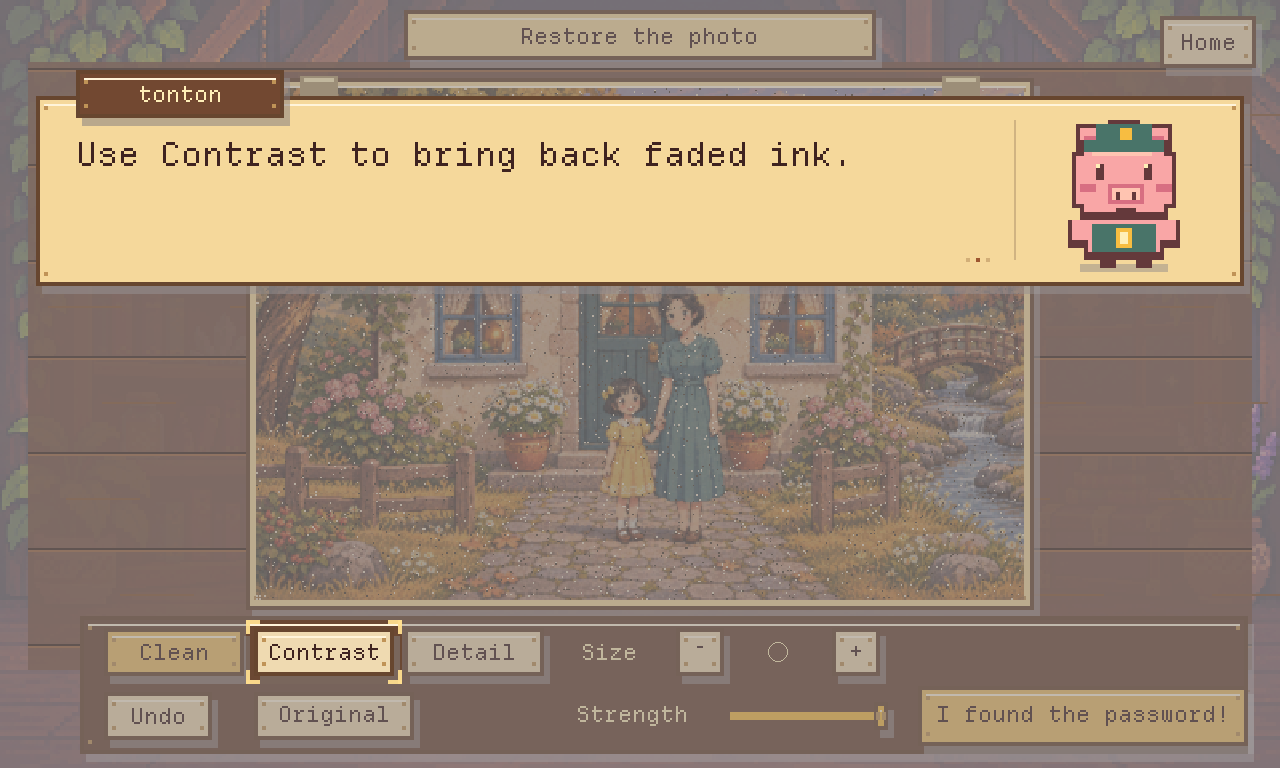
\includegraphics[width=\linewidth]{tool-guide.png}\\[3pt]
{\small (a) A focused tool explanation.}
\end{minipage}\hfill
\begin{minipage}[t]{0.49\linewidth}\centering
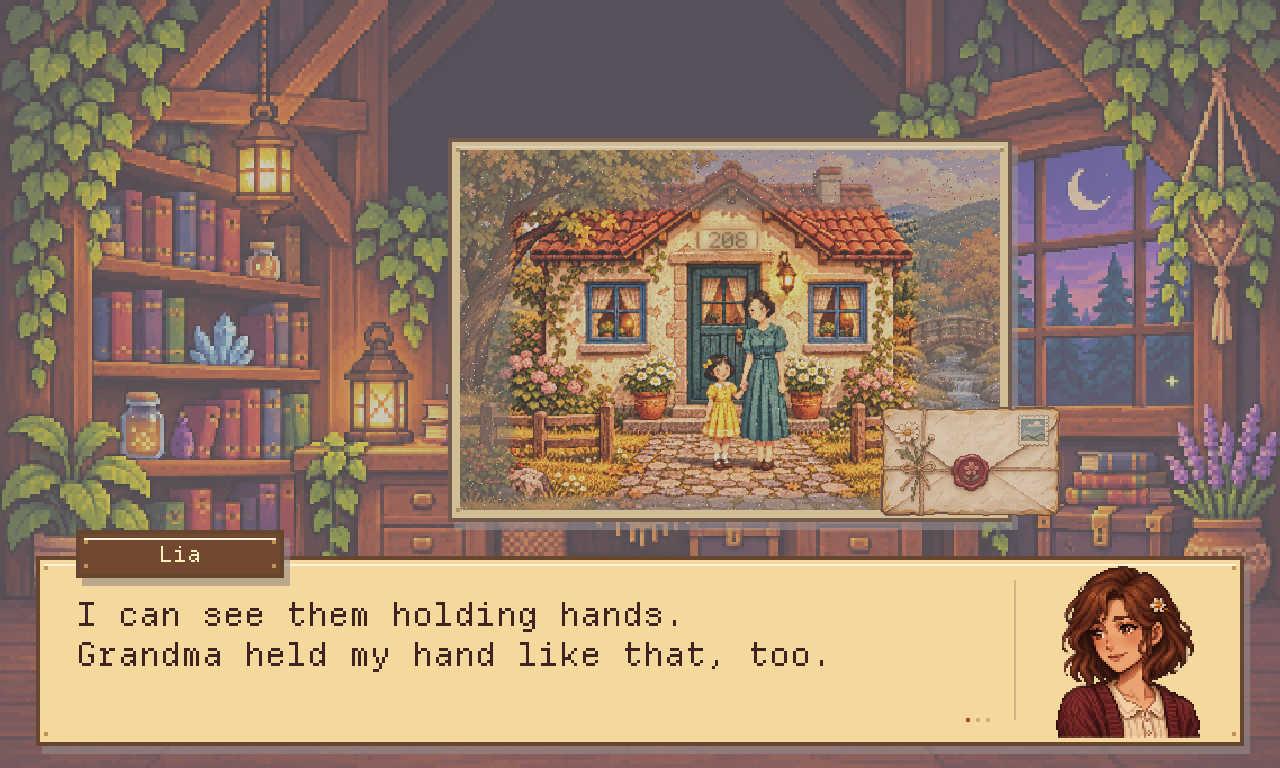
\includegraphics[width=\linewidth]{lia-response.png}\\[3pt]
{\small (b) Lia responds to the repair.}
\end{minipage}\par
\refstepcounter{reportfigure}{\small Figure \thereportfigure. Guidance explains an action; the ending acknowledges its result.}
\end{center}

\subsection{Separated responsibilities and explicit state}
\begin{center}\small
\begin{tabular}{@{}p{46mm}p{117mm}@{}}
\toprule
File / component & Responsibility\\
\midrule
\code{ofApp.cpp/.h} & Screen state, rendering, input routing, camera lifecycle and native interaction QA.\\
\code{StoryScript.h} & Dialogue, character expressions, tutorial focus and explicit story events.\\
\code{HomewardGame.h} & \code{BrushRepair}, \code{DigitReader}, \code{PalmGuide} and \code{Maze}; testable without the graphical interface.\\
\code{HandInput.h}\newline \code{tracker.py} & Process communication, validated palm messages, frame previews and model inference.\\
\code{CameraAccess.*}\newline \code{PixelGrid.h}\newline \code{Tonton.h} & macOS permission handling, viewport conversion and the helper's pixel animation.\\
\code{tests/}, \code{scripts/} & Regression checks, dependency setup, configuration and build commands.\\
\bottomrule
\end{tabular}\end{center}

Enums distinguish screens, filter tools and movement directions. Explicit
Envelope and Letter states enforce the reveal order, while story cues trigger
the doorbell, handover and departure once on entering a dialogue. The Photo
overlay intercepts input before it can reach the underlying lock or map.

At handover, \code{repair.image()} creates an independent snapshot. Lia's personal
response is selected if more than 45\% of a fixed family-region rectangle has
grayscale absolute colour difference above 6 relative to the damaged image.
This measures visible editing, not face recognition or restoration quality.
The same snapshot is exported by \code{imwrite}; no unpainted region is repaired
automatically. Errors cover missing resources, camera startup and PNG writes.
Shared formatting uses four-space indentation and a 100-column limit. State names
describe their purpose; comments explain filter order and recentering. Unused
prototype levels and optical-flow/pinch controls have been removed.

\clearpage
\section{Validation, results and limitations}
\subsection{Measured results}
Validation combines deterministic algorithm tests, scripted interaction tests
and checks of camera startup and restart. The Homeward suite passed 789
assertions, viewport tests passed five assertions, and Python palm tests passed
two tests. Repeated path and frame checks are included in these totals.
The table reports specific results rather than
treating assertion counts as a quality score.

\begin{center}\small
\begin{tabular}{@{}p{39mm}p{124mm}@{}}
\toprule
Check & Result and interpretation\\
\midrule
Faded house number & Mean background-minus-ink intensity rose from 13.66 to 80.17 on an 8-bit grayscale scale after all three default-strength filters. The deterministic test uses the game's pixel-digit pattern and fading procedure.\\
Digit holdout & 2,369 of 2,500 held-out OpenCV samples were correctly classified: 94.76\%. The split is by sheet columns, not a verified split by writer.\\
Mouse handwriting & Mouse-style 2, 0 and 8 were recognised. All nine two-loop 8 variants were read as 8 in the recorded run (stroke widths 3, 5, 8 pixels; tilts $-12$, $0$, $12$ degrees).\\
Hand input rules & Synthetic palm sequences checked centre arming, a single command per hold, diagonal rejection, blocked directions and reset after loss.\\
Map routes & The shortest solution uses eight commands. Every reachable stopping point was checked for a route to the goal; corridor moves cannot pass a turn or fork automatically.\\
Real camera lifecycle & Native QA received 22 preview frames on first start and 19 after closing Photo and restarting. Both runs released the camera; no camera images were saved.\\
\bottomrule
\end{tabular}\end{center}

For the plate measurement, $\Delta=\overline{Y}_{\mathrm{background}}-
\overline{Y}_{\mathrm{ink}}$ uses known masks only during evaluation.
The filtering pipeline never receives these masks. The increase measures clue
contrast, not OCR accuracy or general restoration quality.

\begin{center}
\begin{minipage}[t]{0.49\linewidth}\centering
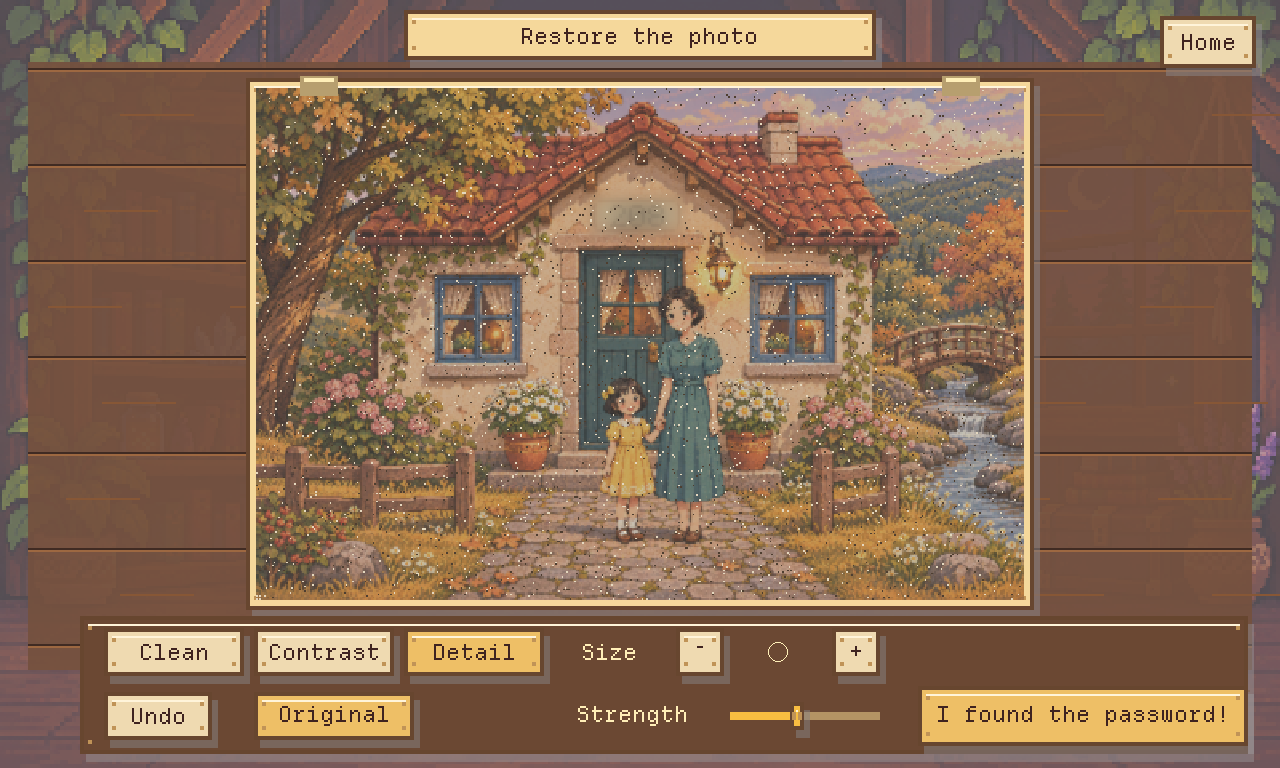
\includegraphics[width=\linewidth]{before.png}\\[3pt]
{\small (a) Original held: damaged observation.}
\end{minipage}\hfill
\begin{minipage}[t]{0.49\linewidth}\centering
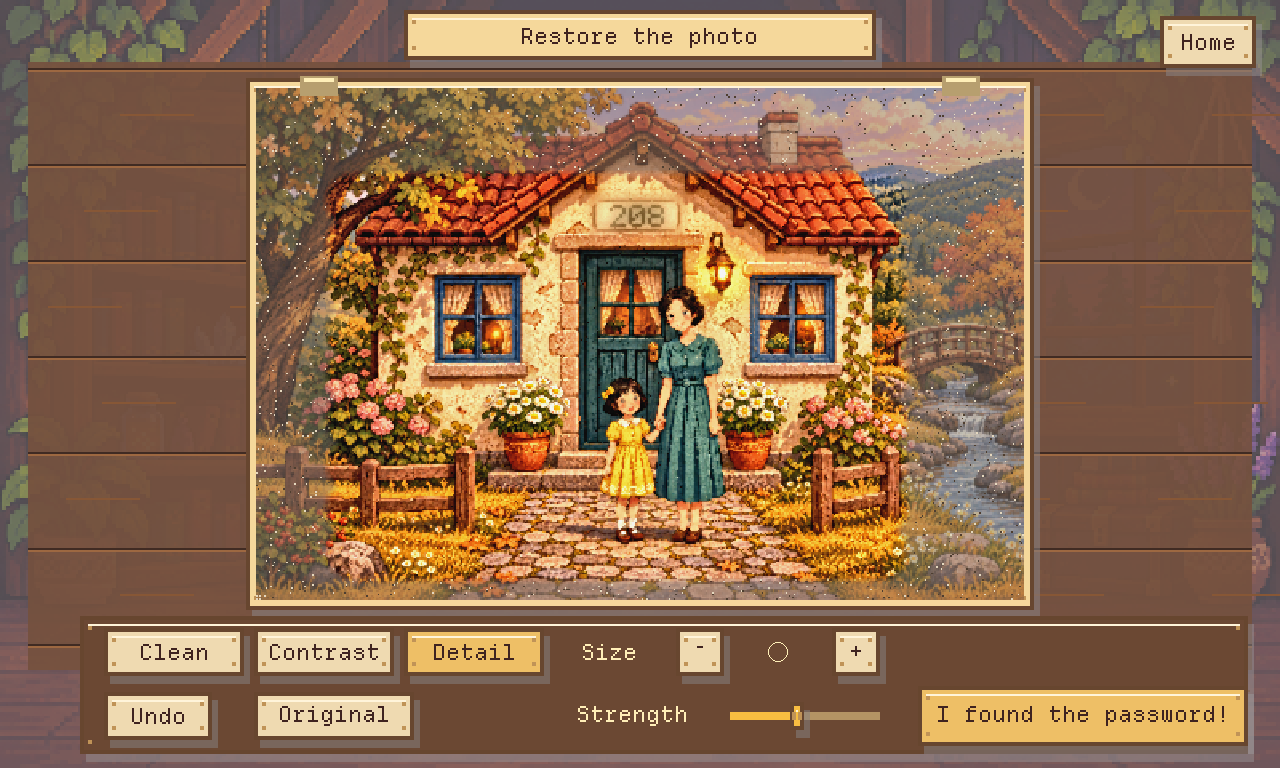
\includegraphics[width=\linewidth]{case1.png}\\[3pt]
{\small (b) The same QA session's local repair.}
\end{minipage}\par
\refstepcounter{reportfigure}{\small Figure \thereportfigure. Damaged and repaired views from a native application QA run.}
\end{center}

\subsection{End-to-end behaviour and practical limits}
Native QA drives real mouse callbacks for painting and handwriting, opens the
envelope, checks both Photo views, and completes the story. It verifies that
photo-view clicks cannot edit the picture, clear handwriting or move the letter.
The returned snapshot and exported PNG match the player's repair exactly,
including deliberately unpainted areas. Automated maze completion uses arrow
keys; camera connection tests do not establish human gesture accuracy.

The game currently has one fixed story, photograph, password and map, limiting
replayability. Filtering can amplify noise; unfamiliar handwriting and hand
occlusion can cause recognition failures. The correction controls and input
resets help recovery but do not remove these limits. No user study or latency
benchmark has been conducted. The next evaluation should measure password
corrections and unintended moves with new players under different lighting.

\clearpage
\section{Reproduction and course connection}
\subsection{Build and run}
The application was built and checked on macOS with openFrameworks 0.12.1 and
Xcode. The C++ project uses the bundled \code{ofxOpenCv} addon; the camera worker
uses Python 3.11 or later with versions pinned in \code{requirements-camera.txt}.
From the project directory:
{\small\begin{verbatim}
./scripts/configure.sh /absolute/path/to/of_v0.12.1_osx_release
./scripts/setup-camera.sh
./scripts/build.sh
open build/Build/Products/Release/MirrorArchive.app
\end{verbatim}}
The setup script creates a local virtual environment. The hand model is included
in \code{bin/data/hand/}. After dependency setup the game works offline. Keep
the app within the project folder, or set \code{MIRROR\_PYTHON} to the configured
Python interpreter if moving it elsewhere. Allow camera access when requested.
Source files, \code{bin/data}, dependency specifications and build scripts are
needed to reproduce the application, together with the Xcode project files;
build caches and the virtual environment
do not need to be submitted.

\subsection{What comes from the course, and what was added}
Median and Gaussian filtering, contrast, histogram reasoning, blending and GUI
controls follow the image-processing lectures and tutorial~\cite{basic,tutorial}.
The brush interaction develops the local-filtering idea used in Assignment 1
with separate masks, feathering, strengths and undo. kNN is covered in the
special-topic lecture~\cite{classification}. The digit normalisation and HOG
descriptor extend it using OpenCV's OCR examples~\cite{knn,svm}. The pretrained
hand model and palm dwell rules are an additional tracking implementation.

\begingroup\small\raggedright
\begin{thebibliography}{8}
\setlength{\itemsep}{3pt}
\bibitem{basic} K. Zhu, \textnormal{Image Formation, Processing, Filtering}, CityUHK CS4187 lecture slides, 2026/27. \code{02\_BasicImage\_2627A.pdf}, pp. 29--36, 58, 114--119, 131, 134--139.
\bibitem{tutorial} K. Zhu, \textnormal{openFrameworks \& Basic Image Processing}, CityUHK CS4187 tutorial, 2026/27. \code{03\_Tutorial\_ImageProcessing.pdf}, pp. 53--55, 77, 84, 97.
\bibitem{classification} CityUHK CS4187, \textnormal{Machine Learning for Image Classification}, special-topic lecture, 2026. \code{CS4187\_special\_topic\_2026.pdf}, p. 22 (k-nearest neighbour classifier).
\bibitem{filtering} OpenCV, \textnormal{Smoothing Images}. \url{https://docs.opencv.org/4.x/d4/d13/tutorial_py_filtering.html}.
\bibitem{clahe} OpenCV, \textnormal{Histograms -- 2: Histogram Equalization}. \url{https://docs.opencv.org/4.x/d5/daf/tutorial_py_histogram_equalization.html}.
\bibitem{knn} OpenCV, \textnormal{OCR of Hand-written Data using kNN}, including the \code{digits.png} dataset. \url{https://docs.opencv.org/4.x/d8/d4b/tutorial_py_knn_opencv.html}.
\bibitem{svm} OpenCV, \textnormal{OCR of Hand-written Data using SVM}, deskewing and HOG example. \url{https://docs.opencv.org/4.x/dd/d3b/tutorial_py_svm_opencv.html}.
\bibitem{hand} Google, \textnormal{MediaPipe Hand Landmarker, Python guide}. \url{https://ai.google.dev/edge/mediapipe/solutions/vision/hand_landmarker/python}.
\end{thebibliography}
Online references accessed 23 November 2026. Lecture page numbers refer to PDF pages.
\endgroup
\end{document}
